The MiniMax algorithm is a decision rule algorithm for minimizing the possible
loss for a worst case (maximum loss) scenario in a zero sum game for 2 (or more)
players who play in turns.

The algorithm builds a game tree, where each tree node represents a game state
and the children represent the possible game moves that can be made by either
player 1 or player 2.  An evaluation function is used to compute the score of
the game for each leaf of the tree. A node is a leaf when the game state can no
longer be expanded. Finally, the algorithm recursively minimizes or maximizes
the scores of each node. To select the best move for player 1, the algorithm
picks the move maximized at the root node.

Figure~\ref{code:coord:minimax} shows LM's code for the MiniMax program using
coordination facts. The program starts with a root node (with the initial game state) that
is expanded with the available moves at each level. The graph of the program is
dynamic since nodes are created and then deleted once they are no longer
needed. The latter happens when the leaf scores are computed or when a node
fully minimizes or maximizes the children scores. When the program ends, only
the root node has facts in its database.

The first two rules in
lines~\ref{line:coord:minimax_play1}-\ref{line:coord:minimax_play2} check if the
current game is final, namely, if a player has won or the game drew: the first
rule generates the score for the final state while the second expands the game
state by generating all the possible plays for player \code{NextPlayer}.

The expansion rules create the children for the current node and are
implemented in
lines~\ref{line:coord:minimax_expand1}-\ref{line:coord:minimax_expand2}. The
first two rules create either a \code{maximize} or \code{minimize} fact that
will either maximize or minimize the scores of the children nodes.  The third
and fourth expansion rules simulate a player move and, for that, create a new
node \code{B} using the \code{exists} language construct. We link \code{B} with
\code{A} using \code{parent(B, A)} and kickstart the recursive expansion of node
\code{B} by deriving a \code{play} fact. Finally, the rule in
lines~\ref{line:coord:minimax_expand11}-\ref{line:coord:minimax_expand2} is for
the case when the current player cannot play in the current game position. The
full proof of correctness is presented in
Appendix~\ref{appendix:proofs:minimax}.

\iffalse
\begin{wrapfigure}{r}{0.4\textwidth}
   \begin{center}
      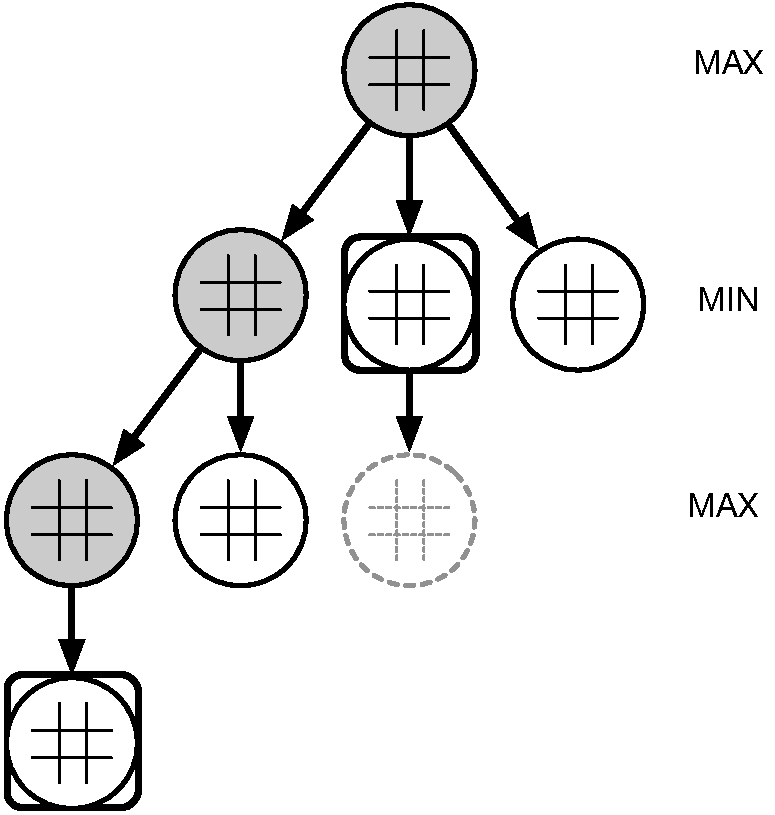
\includegraphics[width=0.9\linewidth]{figures/coordination/minimax_tree}
   \end{center}
   \caption{Expanding the MiniMax tree using coordination. By prioritizing
      deeper nodes, threads are forced to expand the tree using a depth-first
      approach, which is superior since there is no need to expand the whole
      tree before computing the node scores.}
   \label{fig:coord:minimax}
\end{wrapfigure}
\fi

As noted in Section~\ref{sec:coord:fifo}, LM's default scheduler uses a FIFO
approach, which results in a breadth-first expansion of the MiniMax tree. This
results in $\mathcal{O}(n)$ space complexity, where $n$ is the number of nodes
in the tree, since the tree must be fully expanded before the scores at the
leaves are actually computed.  With coordination, we set the priority of a node
to be its depth (lines~\ref{line:coord:minimax_coord1} and
\ref{line:coord:minimax_coord2}) so that the tree is expanded in a depth-first
fashion, leading to $\mathcal{O}(d t)$ memory complexity, where $d$ is the depth
of the tree and $t$ is the number of threads. Since threads prioritize deeper
nodes, the scores of the first leaves are immediately computed and then sent to
the parent node. At this point, the leaves are deleted and reused for other
nodes in the tree, resulting in minimal memory usage.  As an example, consider a
system with 2 threads, $T_1$ and $T_2$, where $T_1$ first expands the root node
and then the first child. Since $T_2$ is idle, it steals half of the root's
children nodes and starts expanding one of the nodes in a depth-first fashion.

\begin{figure}[ht]
\begin{Verbatim}[numbers=left,commandchars=\\\{\},fontsize=\scriptsize]
type list int game.\hfill// Type declaration
type linear parent(node, node).\hfill// Predicate declaration
type linear score(node, int, int).
type linear new-score(node, int, int).
type linear minimize(node, int, int, int).
type linear maximize(node, int, int, int).
type linear expand(node, game FirstPart, game SecondPart, int Descendants, int Player, int Play, int Depth).
type linear play(node, game Game, int Player, int Play, int Depth).

const root-player = 1. const initial-game = [...].\hfill// Constant declaration: player and initial game state
fun next(P : int) : int = if P = 1 then 2 else 1 end.\hfill// Function declaration: select next player

play(A, Game, NextPlayer, LastPlay, Depth),\label{line:coord:minimax_play1}\label{line:coord:minimax_play11}\hfill// Rule 1: ending game state
Score = minimax_score(Game, NextPlayer, root-player), Score > 0
   -o score(A, Score, LastPlay).\label{line:coord:minimax_play12}

play(A, Game, NextPlayer, LastPlay, Depth),\label{line:coord:minimax_play21}\hfill// Rule 2: expand state
0 = minimax_score(Game, NextPlayer, root-player)
   -o expand(A, [], Game, 0, NextPlayer, LastPlay, Depth).\label{line:coord:minimax_play2}\label{line:coord:minimax_play22}

expand(A, Game, [], N, Player, Play, \underline{Depth}), Player = root-player\label{line:coord:minimax_expand1}\label{line:coord:minimax_rule11}\hfill// Rule 3: maximize node
   -o maximize(A, N, -00, 0).\label{line:coord:minimax_rule12}

expand(A, Game, [], N, Player, Play, \underline{Depth}), Player <> root-player\label{line:coord:minimax_rule21}\hfill// Rule 4: minimize node
   -o minimize(A, N, +00, 0).\label{line:coord:minimax_rule22}

expand(A, First, [0 | Xs], N, Player, Play, \underline{Depth}), Depth >= 5\label{line:coord:minimax_rule31}\hfill// Rule 5: create static child node
   -o exists B. (\underline{set-static(B)},\label{line:coord:minimax_coord1}
       \underline{set-default-priority(B, float(Depth + 1))},\label{line:coord:minimax_coord2}
       play(B, Game ++ [P | Xs], next(P), length(First), \underline{Depth + 1}), parent(B, A).
       expand(A, First ++ [0], Xs, N + 1, Player, Play, \underline{Depth})).\label{line:coord:minimax_rule32}

expand(A, First, [0 | Xs], N, Player, Play, \underline{Depth}), Depth < 5\label{line:coord:minimax_rule41}\hfill// Rule 6: create child node
  -o exists B. (\underline{set-default-priority(B, float(Depth + 1))},\label{line:coord:minimax_coord3}
       play(B, Game ++ [P | Xs], next(P), length(First), \underline{Depth + 1}), parent(B, A),
       expand(A, First ++ [0], Xs, N + 1, Player, Play, \underline{Depth})).\label{line:coord:minimax_rule42}

expand(A, First, [C | Xs], N, Player, Play, \underline{Depth}) C <> 0\label{line:coord:minimax_expand11}\label{line:coord:minimax_rule51}\hfill// Rule 7: next game play
  -o expand(A, First ++ [C], Xs, N, Player, Play, \underline{Depth}).\label{line:coord:minimax_expand2}\label{line:coord:minimax_rule52}

score(A, Score, BestPlay), parent(A, B) -o new-score(B, Score, BestPlay).\label{line:coord:minimax_new}\hfill// Rule 8: sending score to parent node

new-score(A, Score, Play), minimize(A, N, Current, BestPlay), Current > Score\label{line:coord:minimax_minimize1}\hfill// Rule 9: keep current score
   -o minimize(A, N - 1, Score, Play).

new-score(A, Score, Play), minimize(A, N, Current, BestPlay), Current <= Score\hfill// Rule 10: select new best
   -o minimize(A, N - 1, Current, BestPlay).

minimize(A, 0, Score, BestPlay) -o score(A, Score, BestPlay).\label{line:coord:minimax_minimize2}// Rule 11: score minimized

new-score(A, Score, Play), maximize(A, N, Current, BestPlay), Current < Score\label{line:coord:minimax_maximize1}\label{line:coord:minimax_maximize_rule11}\hfill// Rule 12: keep current score
   -o maximize(A, N - 1, Score, Play).\label{line:coord:minimax_maximize_rule12}

new-score(A, Score, Play), minimize(A, N, Current, BestPlay), Current >= Score\label{line:coord:minimax_maximize_rule21}\hfill// Rule 13: select new best
   -o maximize(A, N - 1, Current, BestPlay).\label{line:coord:minimax_maximize_rule22}

maximize(A, 0, Score, BestPlay) -o score(A, Score, BestPlay).\label{line:coord:minimax_maximize2}\hfill// Rule 14: score maximized

play(@0, initial-game, root-player, 0, 1).\label{line:coord:minimax_axiom}\hfill// Initial fact
\end{Verbatim}
\caption{LM code for the MiniMax program.}
\label{code:coord:minimax}
\end{figure}

We also take advantage of memory locality by using \code{set-static}
(line~\ref{line:coord:minimax_coord2}), so that nodes after a certain level are
   not stolen by other threads. While this is not critical for performance in
   shared memory systems where node stealing is fairly efficient, we expect that
   such coordination to be critical in distributed systems.

The rest of the program contains rules for maximizing and minimizing scores
(lines~\ref{line:coord:minimax_minimize1}-\ref{line:coord:minimax_maximize2}),
through the retraction of \code{new-score} incoming facts.

\begin{figure}[ht]
   \begin{center}
      \begin{tabular}{c | c || c c | c c | c c} \hline
	 \multirow{2}{*}{\textbf{Size}} & \multirow{2}{*}{\textbf{Threads}} & \multicolumn{2}{c|}{\textbf{Average}} & \multicolumn{2}{c|}{\textbf{Final}} & \multicolumn{2}{c}{\textbf{\# Malloc}}\\
	 & & Regular & Coord & Regular & Coord & Regular & Coord\\ \hline \hline
\multirow{7}{*}{Small}  & 1 &  1794.8MB & 38KB &  33KB & 33KB &  42 & 11\\
 & 2 &  869.4MB & 35KB &  64KB & 65KB &  80 & 22\\
 & 4 &  436.2MB & 34KB &  128KB & 129KB &  152 & 44\\
 & 8 &  198.6MB & 32KB &  254KB & 258KB &  284 & 88\\
 & 16 &  65.3MB & 33KB &  508KB & 514KB &  513 & 172\\
 & 24 &  40.5MB & 32KB &  761KB & 770KB &  742 & 256\\
 & 32 &  24.4MB & 32KB &  1014KB & 1022KB &  953 & 335\\
\hline
\multirow{7}{*}{Big}  & 1 &  14.5GB & 43KB &  33KB & 33KB &  48 & 12\\
 & 2 &  7.2GB & 35KB &  64KB & 65KB &  92 & 24\\
 & 4 &  2.4GB & 36KB &  128KB & 130KB &  172 & 45\\
 & 8 &  1748.3MB & 33KB &  254KB & 258KB &  331 & 89\\
 & 16 &  665.10MB & 34KB &  508KB & 515KB &  620 & 177\\
 & 24 &  271.3MB & 35KB &  761KB & 771KB &  871 & 265\\
 & 32 &  193.5MB & 34KB &  1014KB & 1027KB &  1123 & 353\\
\hline
\end{tabular}

   \end{center}

   \caption{Comparing the memory usage of the regular and coordinated MiniMax
   programs.}
   \label{results:memory_minmax}
\end{figure}

In Table~\ref{results:memory_minmax} we compare the memory usage of the
coordinated MiniMax program against the regular MiniMax program. The
\textbf{Average} column presents the average memory usage during the lifetime of
the program, the \textbf{Final} indicates the amount of memory used at the end
of the program, while the \textbf{\# Malloc} column represents the number of
calls made to the \code{malloc} function by the threaded allocator. The
coordinated version uses significantly less memory than the regular version. As
the number of the threads increases, the average memory usage of the regular
version decreases because there are more threads that are able to complete
different parts of the tree at the same time. The same thing happens for the
coordinated version, but at a much smaller scale since threads are exploring the
tree in a depth-first fashion. Finally, as expected, there is also a large
reduction in the number of \code{malloc}'s called by the threaded allocator in
the coordinated version.

The run time and scalability results are presented in
Fig.~\ref{fig:coordination:results_minmax}. There is a clear performance
improvement when coordinating the MiniMax program due to the low memory usage.
The Big dataset needs only 5 threads to reach the performance of the
sequential C++ program and, when using 32 threads, the LM program is more than
four times faster than the C++ version. The use of coordination facts allows us
to improve the execution of this declarative program and make it run
significantly faster than it would be otherwise.

\begin{figure}[]
        \centering
        \begin{subfigure}[b]{\plotsize\textwidth}
           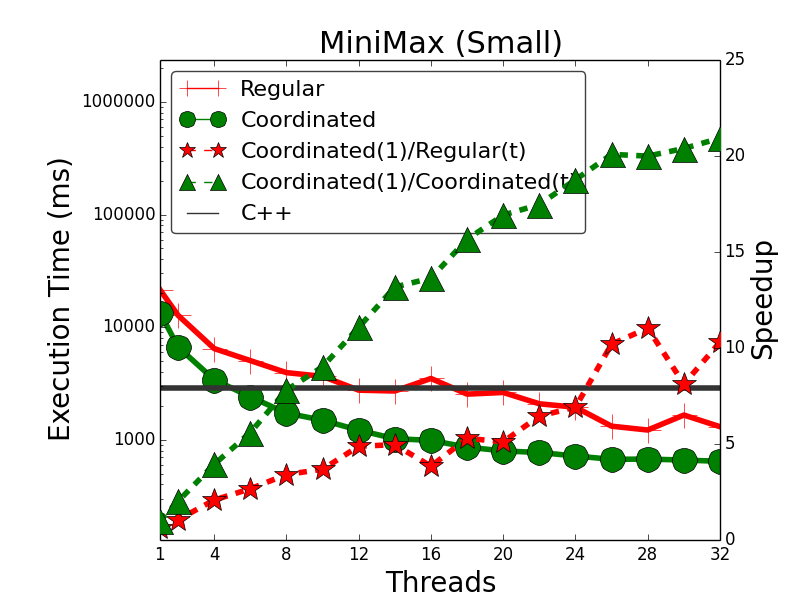
\includegraphics[width=\textwidth]{experiments/coordination/cmp-min-max-tictactoe-small.png}
           \label{fig:coordination:coord_minimax_small}
        \end{subfigure}
        ~
        \begin{subfigure}[b]{\plotsize\textwidth}
           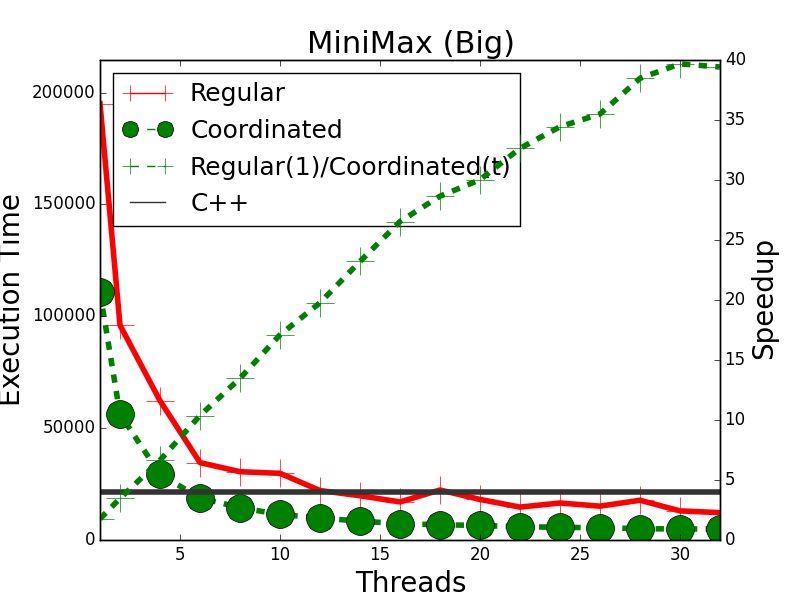
\includegraphics[width=\textwidth]{experiments/coordination/cmp-min-max-tictactoe-big.png}
           \label{fig:coordination:coord_minimax_big}
        \end{subfigure} \\

        \caption{Scalability for the MiniMax program when using coordination.}

        \label{fig:coordination:results_minmax}
\end{figure}

\clearpage
